% Klassische Darstellung eines Feed-Forward-Netzes: Kreise als Neuronen, Linien als Gewichte.
% Bauen: lualatex d_t09_netz_klassisch.tex && pdftoppm -png -scale-to-x 2400 -scale-to-y -1 -singlefile d_t09_netz_klassisch.pdf d_t09_netz_klassisch
\documentclass[tikz,border=0pt]{standalone}
\usepackage{fontspec}
\setmainfont{Helvetica Neue}
\setsansfont{Helvetica Neue}
\usetikzlibrary{calc,backgrounds}

\definecolor{paper}{HTML}{F4F7FB}
\definecolor{ink}{HTML}{183B66}
\definecolor{muted}{HTML}{5A6B82}
\definecolor{soft}{HTML}{B9C6D8}
\definecolor{accent}{HTML}{2459A6}
\definecolor{tint}{HTML}{E3EAF5}

\begin{document}
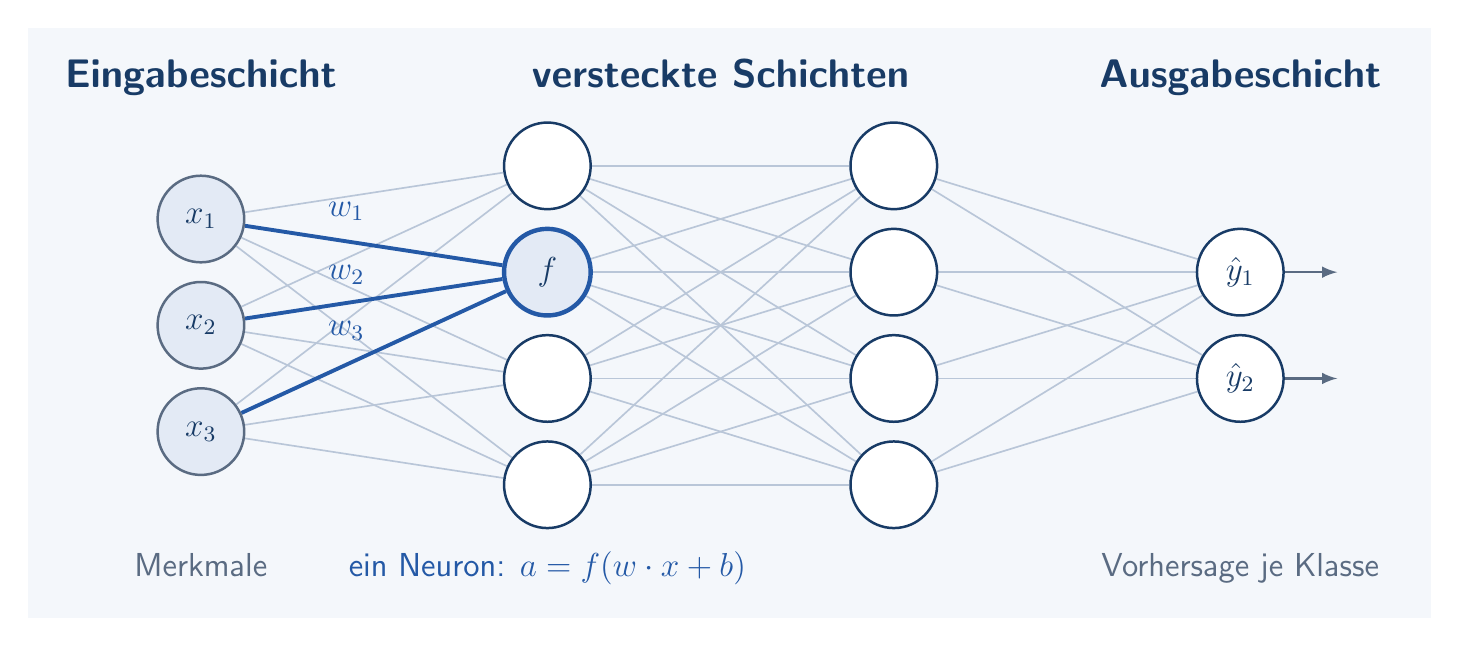
\begin{tikzpicture}[
    x=4.4cm, y=1.35cm,
    neuron/.style={circle, draw=ink, fill=white, line width=0.9pt, minimum size=1.1cm,
                   inner sep=0pt, font=\sffamily\large, text=ink},
    input/.style={neuron, draw=muted, fill=tint},
    focus/.style={neuron, draw=accent, fill=tint, line width=1.6pt},
    edge/.style={draw=soft, line width=0.6pt},
    fedge/.style={draw=accent, line width=1.4pt},
    layer/.style={font=\sffamily\bfseries\Large, text=ink, text height=1.6ex, text depth=0.5ex},
    sub/.style={font=\sffamily\large, text=muted, text height=1.6ex, text depth=0.5ex},
  ]

  % Papierfläche zuerst, damit sie hinter den Verbindungen liegt
  \begin{scope}[on background layer]
    \fill[paper] (-0.5, -2.75) rectangle (3.55, 2.8);
  \end{scope}

  % Neuronen je Schicht, senkrecht um y=0 zentriert
  \foreach \i in {1,2,3}   \node[input]  (x\i) at (0, {2 - \i}) {$x_\i$};
  \foreach \i in {1,...,4} \node[neuron] (h\i) at (1, {2.5 - \i}) {};
  \foreach \i in {1,...,4} \node[neuron] (g\i) at (2, {2.5 - \i}) {};
  \foreach \i in {1,2}     \node[neuron] (o\i) at (3, {1.5 - \i}) {$\hat{y}_\i$};
  \node[focus] (h2) at (1, 0.5) {$f$};

  % Verbindungen hinter den Kreisen
  \begin{scope}[on background layer]
    \foreach \i in {1,2,3} \foreach \j in {1,3,4} \draw[edge] (x\i) -- (h\j);
    \foreach \i in {1,...,4} \foreach \j in {1,...,4} \draw[edge] (h\i) -- (g\j);
    \foreach \i in {1,...,4} \foreach \j in {1,2} \draw[edge] (g\i) -- (o\j);
    \foreach \i in {1,2,3} \draw[fedge] (x\i) -- (h2);
  \end{scope}

  % Gewichte am hervorgehobenen Neuron
  \node[sub, text=accent] at ($(x1)!0.42!(h2) + (0, 0.30)$) {$w_1$};
  \node[sub, text=accent] at ($(x2)!0.42!(h2) + (0, 0.28)$) {$w_2$};
  \node[sub, text=accent] at ($(x3)!0.42!(h2) + (0, 0.34)$) {$w_3$};

  % Ausgabepfeile
  \foreach \i in {1,2} \draw[draw=muted, line width=0.9pt, -latex] (o\i) -- ++(0.28, 0);

  % Beschriftung der Schichten
  \node[layer] at (0, 2.3) {Eingabeschicht};
  \node[layer] at (1.5, 2.3) {versteckte Schichten};
  \node[layer] at (3, 2.3) {Ausgabeschicht};
  \node[sub] at (0, -2.3) {Merkmale};
  \node[sub, text=accent] at (1, -2.3) {ein Neuron: $a = f(w \cdot x + b)$};
  \node[sub] at (3, -2.3) {Vorhersage je Klasse};

\end{tikzpicture}
\end{document}
